\chapter{Osterwalder Business Model Ontology}
We have decided to use Osterwalder Business Model Ontology for the analysis of the case. Osterwalder defines a business model like this "A business model describes the rationale of how an organization creates, delivers, and capture values" \cite{osterwalder}. Osterwalder came up with a way to describe business models through nine building blocks. Going through these building blocks allows us to describe and think through the business model of any enterprise by covering four main areas of a business:  Product, Customer Interface, Infrastructure Management and Financial Aspects. The nine different building blocks are: Customer Segments, Value Propositions, Channels, Customer Relationships, Revenue Streams, Key Resources, Key Activities, Key Partnerships and Cost Structure.The nine business model elements are the core of the model, see Figure \ref{fig:TheBusinessModelCanvas}. In this chapter we will go through every of the nine building blocks in more detail.


\begin{figure}[h]
\caption[The Business Model Canvas]{The Business Model Canvas [modified from \cite{osterwalder}]}
\label{fig:TheBusinessModelCanvas}
\begin{center}
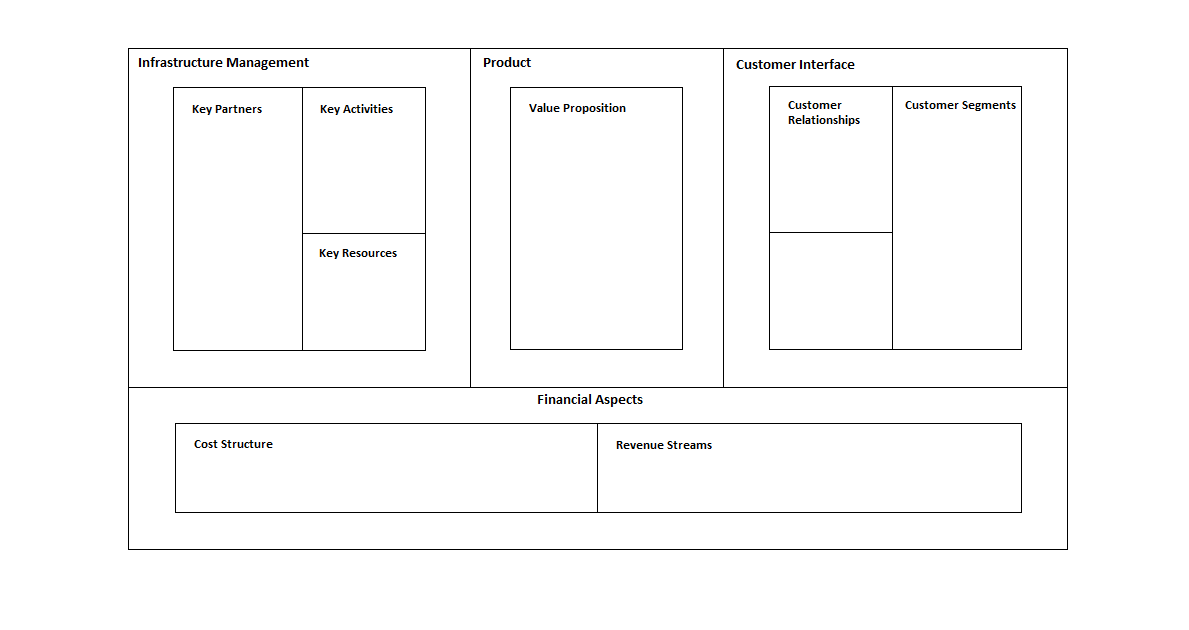
\includegraphics[scale=0.6]{osterwaldersbmmodified}
\end{center}
\end{figure}
\newpage
\section{Product}
Product is what the company offers to its customer and how it differentiates itself from its customers. This area covers the building block Value Proposition \cite{osterwalderthesis}.

\subsection{Value Proposition}
Osterwalder's definition is: "The Value Propositions Building Block describes the bundle of products and services that create value for a specific Customer Segment" \cite{osterwalder}. This is what the organization actually offers to their customer or customer segments and are suppose to satisfy the customers needs. It might be different value propositions for the different customer segments. The values can be both quantitative and qualitative, meaning that the value can rely on for example price or on design. The value propositions have to be so good that the organization's defined customer segments turn to them over another company. It can be either something new, an improvement of already existing products or services, customizing products and services or simply just helping a customer to get a certain job done. Something to also consider is design and brand. These two aspects are more important in some type of products than other. With the Value Propositions it is also important to compare price levels with their competitors. A common way to satisfy the needs of the customer is to offer them the same value to a lower price. The firm can also keep-up with the market price, offer luxury goods to a higher price or simply offer a Value Proposition for free. For the latter, the model is based on an other source of income, for example from advertising. \\ \\
There are different ways of creating value for the Customer. By reducing the cost, this will for most customer be experienced as valuable. Also reducing the risk when buying something, by for example offering them one-year guarantee is very satisfactory for customers. Other ways of creating value are to make products and services available for customers that did not have access to them before and to make products and services easier and more convenient to use.


\section{Customer Interface}
Customer Interface covers everything that have to to with customers: who they are, what kind of relationship the firm has with them and how the firm reach out to them. The three building block covered by this area are thus: Customer, Channel and Customer Relationships, described below \cite{osterwalderthesis}.

\subsection{Customer Segments}
Osterwalder's definition is: "The Customer Segments Building Block defines the different groups of people or organizations an enterprise aims to reach and serve" \cite{osterwalder}. To make a good business, you have to understand who the business are meant to create value for, which is all about segmentation. It is important to carefully choose the most important customers and to focus on them and their needs. A business can have more than one customer segment, but they can not always serve all segments. Therefore a careful valuation has to be done to choose this organizations most important segment(s).  \\ \\
A firm can deliver a value Proposition to different types of Customer Segments. They can choose to not distinguish between customer segments and rather focus on the mass market, they can distinguish their customers into segments with slightly different needs or problems, or sharpen it even more by targeting a niche market with specialized customers. The firm can also serve unrelated Customer Segments or even independent Customer segments. 

\subsection{Channels}
Osterwalder's definition is: "The Channel Building Block describes how a company communicates with and reaches its Customer Segments to deliver a Value Proposition" \cite{osterwalder}. This is about finding the best and most cost-efficient way of reaching the right customer, at the right place and right time. We distinguish between five channel phases: 
Awareness ---> Evaluation ---> Purchase ---> Delivery ---> After Sales
It is important for an organization to think about how the customers want to be reached in all of these phases and how the channels can be integrated with the customers routines. The way the organization communicates with the customers is an important role in the customer experience. The value proposition can be delivered either directly, through for example sales force, or indirectly through intermediaries. The direct and/or indirect channels are decomposed into Link(s). \\ \\ 
Link(s) describes each of the different ways the firm reach out to its customer, either direct or indirect. The set of Links together describes a Channel. Channel links have the potential for value creation and therefore it contributes to a company's Value Proposition \cite{osterwalderthesis}. \\ \\
As mention, we can distinguish between five channel phases of a customer's buying cycle, see Figure \ref{fig:BuyingCycle}. A channel should be studied over all these phases.

\begin{figure}[h]
\caption[BuyingCycle]{Buying Cycle}
\label{fig:BuyingCycle}
\begin{center}
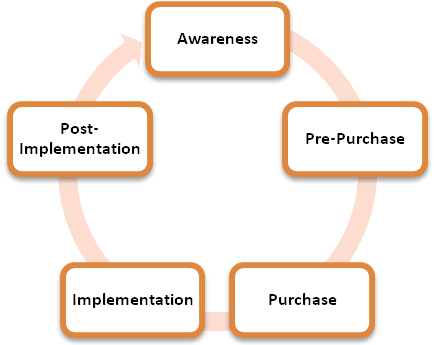
\includegraphics[scale=1.0]{5BuyingStages.png}
\end{center}
\end{figure} 

\newpage
\subsection{Customer Relationships}
Osterwalder's definition is: "The Customer Relationships Building Block describes the types of relationships a company establishes with specific Customer Segments" \cite{osterwalder}. The Customer Relationship is based on customer equity and can be decomposed into several Relationships Mechanisms. The customer relationship is very important for the customers overall experience. This can range from personal assistance, where a real customer representative communicates with the customer, to a more automated service, where typically the customer helps himself,  to a more community based service that allows customer to exchange experiences with each other. For every type of Customer Segments defined, the organization has to keep in mind what kind of relationship the Customer wishes to have. At the same time, the organization has to keep in mind how this relationship is integrated with the rest of their business model and how costly they are. There are three different customer equity goals: customer acquisition, customer retention and boosting sales (upselling).

\begin{itemize}
\renewcommand{\labelitemi}{$\bullet$}
\item \emph{Acquisition:} A company needs customers to do business. The customer acquisition is a very expensive affair and must be carefully managed and evaluated because the relationship developed with its customers will strongly influence the two next equity goals \cite{osterwalderthesis}.
\item \emph{Retention:} “The goal of customer retention is to leverage customer acquisition investments. “<-skrive om.The customer acquisition is usually more expensive than customer retention. Because of this ways to extend the duration of the relationships between the company and its (profitable) customer should be found. High switching costs is an element that can help retention. This means that the cost of ending the relationship and building a new one is so high that the customer does not want to switch \cite{osterwalderthesis}.
\item \emph{Boosting sales (upselling):} This means adding on to your initial sale with additional products and services \cite{osterwalderthesis}.
\end{itemize}

\section{Infrastructure Management}
Infrastructure management describes the companies capabilities and resources that are necessary to deliver the value proposition and maintain customer interface. This block also describes who provides and own the capabilities and resources, as well as who executes the activities and the relationship between them \cite{osterwalderthesis}.

\subsection{Key Resources}
Osterwalder's definition is: "The Key Resources Building Block describes the most important assets required to make a business model work" \cite{osterwalder}. This means all the resources you need to make all the 4 described building blocks work. The resources can be physical (e.g. buildings and machines), intellectual (e.g. brands, patents and copyrights), human (for example in an industry where knowledge is in particular important) and financial (e.g. cash). The company does not need to have all the resources within their organization, they (bedre ord for “de”?) can also be acquired from outside the company. Usually you can link a Resource to one or more Activities (described below).

\subsection{Key Activities}
Osterwalder’s definition is: “The Key Activities Building Block describes the most important things a company must do to make its business model work” \cite{osterwalder}. This means all the actions that have to be done to make all the 4 first building blocks described work and to create and market value and generate profit. The key Activities will depend on what kind of company it is and can be divided into production (e.g. designing, making, and delivering a product), problem solving (e.g. coming up with a solution to a problem), and platform/network (e.g. platform management, service provisioning, and platform promotion). 
Osterwalder distinguish between primary and support activities. Primary activities are involved in the creation of the value proposition and its marketing and delivery. Support activities are the underlying activities that have to be in-place for the primary activities to take place (e.g. firm infrastructure, technology) \cite{osterwalderthesis}.\\ \\
As outlined above, the main purpose of a company is the creation of value that customers are willing to pay for. This value is the outcome of a configuration of inside and outside activities and processes.\\ \\
The value that the company creates is an outcome of a configuration of inside and outside activities and processes. There are three different different types of configurations, value chain, value shop and value network, that all have different primary activities \cite{osterwalderthesis}:

\newpage

\emph{Value Chain:} 

\begin{figure}[h]
\caption[ValueChain]{Value Chain [modified from \cite{osterwalderthesis}]}
\label{fig:ValueChain}
\begin{center}
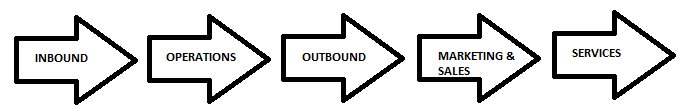
\includegraphics[scale=0.8]{valuechain}
\end{center}
\end{figure}


This is all about how a firm creates value from taking an input, transforming it to the final product (refined output), distribute the product  to the customers and maintain the product. At each step there are added value (e.g. production and manufacturing)

\bigskip

\emph{Value Shop:}

Problem Finding and Acquisition--Problem Solving--Choice--Execution --Control and Evaluation
---------------------------------------------------------------------------------------------------------------------------
(sirkel) (få tak i figur)

This figure describes how a firm can create value for its customers by understanding their problem and finding a solution for it (e.g. consultancies and doctors).

\bigskip

\emph{Value Network:}

\begin{figure}
\caption[ValueNetwork]{Value Network \cite{osterwalderthesis}}
\label{fig:ValueNetwork}
\begin{center}
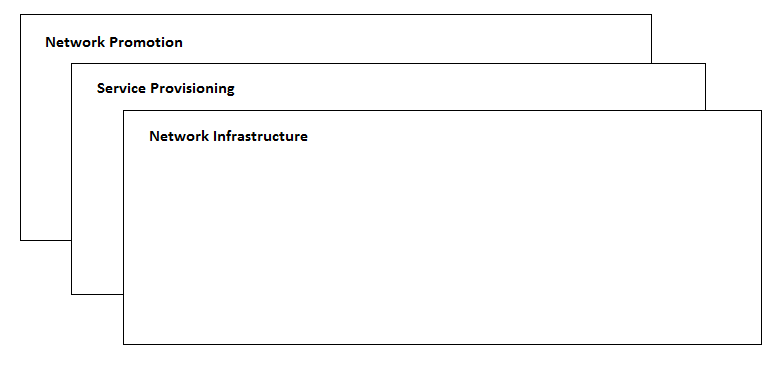
\includegraphics[scale=0.5]{valuenetwork}
\end{center}
\end{figure}

This is about network effects, which means that the more people a network has the more value it gets. (e.g. banks and telecom operators). It consists of getting potential customers to the network, establishing links between customers and billing for value received, and maintaining and running a physical and information infrastructure so it is ready to serve customers requests. 
\newpage
\subsection{Key Partnerships}
Osterwalder’s definition is: “The Key Partnerships Building Block describes the network of suppliers and partners that make the business model work” \cite{osterwalder}. Not always can a company do everything on their own. The motivation for creating partnerships can be divided in three: 
\\
1. \emph{Optimizing their business model:} Sometimes it is not profitable for a company to own all resources and do everything in-house. Cooperating with other firms can reduce costs and optimize the allocation of resources and activities. 
\\
2. \emph{Reduce risk:} In a very competitive market it can be safer to cooperate with the competitors in one area, even though they are competing in another.
\\
3. \emph{Acquire resources:} Usually it is not very profitable for a company to have all resources and to have the knowledge to do all the activities. Cooperating with other firms by buying/lending resources is often more profitable than having everything in-house. 

\section{Financial Aspects}
All of the other blocks already described influence this last block in the framework, thus this block is an outcome of the rest of the business model configuration. This area covers the Revenue Streams and Cost Structure elements \cite{osterwalderthesis}

\subsection{Revenue Streams}
Osterwalder’s definition is: “The Revenue Streams Building Block represents the cash a company generates from each Customer Segment” \cite{osterwalder}. This is where the company earns its money. It is important to keep in mind what the customers are willing to pay, as well as what they are currently paying. A firm can have one or more revenue streams where each revenue stream can have different pricing mechanisms, shown in table blabla. There are several ways of generating revenue streams, including asset sale (e.g. selling a car), usage fee (e.g. customer pays his telecom operator for the minutes he has spend on the phone), subscription fee (e.g. users of Spotify pay a monthly fee to access Spotify Premium), renting (e.g. renting a car for the weekend), licensing (e.g. companies have to pay a license fee to get access to a patented technology), brokerage fee (e.g. a seller earn a commision each time they sell something.. sjekk denne), and advertising (e.g. newspapers take a fee for companies who wants to promote a specific product or service in their newspaper). \\ \\ 
The pricing mechanism chosen is very important and can make a huge difference on how much revenue that is generated. Osterwalder distinguish between two types of pricing mechanisms: fixed and dynamic pricing. 
TABELL: PRICING MECHANISMS s 33 i boka

\subsection{Cost Structure}
Osterwalder’s definition is: “The Cost Structure describes all costs incurred to operate a business model” \cite{osterwalder}. The costs in the business model come from Key Resources, Key Activities and Key Partnerships. The book \cite{osterwalder} defines two cost structures: cost-driven business model, which focus on minimizing costs, and value-driven business model, which are focussing on value creation by for example making personalized services. Despite of if the model is cost-driven or value-driven the costs can have the following structure: fixed costs (e.g. costs stay the same regardless of the volume), variable costs (e.g. costs depends on volume), economies of scale (e.g. less cost as output increases), economies of scope (e.g. less cost due to a larger scope of operations). 
